% !TeX program = pdfLaTeX
\documentclass[12pt]{article}
\usepackage{amsmath}
\usepackage{amsthm}
\usepackage{amssymb}
\usepackage{bbm}
\usepackage{graphicx,psfrag,epsf}
\usepackage{enumerate}
%\usepackage[numbers]{natbib}
\usepackage[nomarkers]{endfloat}
\usepackage{natbib}
\setcitestyle{numbers} 
\makeatletter % Reference list option change
\renewcommand\@biblabel[1]{#1. } % from [1] to 1
\makeatother %

\usepackage{booktabs}
\usepackage{longtable}
\usepackage{array}
\usepackage{adjustbox}
\usepackage{multirow}
\usepackage{subfig}
\usepackage[table,xcdraw]{xcolor}
\usepackage{wrapfig}
\usepackage{float}
%\usepackage{colortbl}
\usepackage[colorlinks]{hyperref}
\hypersetup{
  colorlinks=true,
  citecolor=black,
  linkcolor=black,
  urlcolor=blue}
  
\usepackage{pdflscape}
\usepackage{tabu}
\usepackage{threeparttable}
\usepackage{url} % not crucial - just used below for the URL

\usepackage{etoolbox}% http://ctan.org/pkg/etoolbox
\makeatletter
\patchcmd{\subsection}{\bfseries}{\relax}{}{}% Non-bold \subsection
\patchcmd{\subsubsection}{\bfseries}{\relax}{}{}% Non-bold \subsection
\makeatother


%\pdfminorversion=4
% NOTE: To produce blinded version, replace "0" with "1" below.
\newcommand{\blind}{0}

% DON'T change margins - should be 1 inch all around.
\addtolength{\oddsidemargin}{-.5in}%
\addtolength{\evensidemargin}{-.5in}%
\addtolength{\textwidth}{1in}%
\addtolength{\textheight}{1.3in}%
\addtolength{\topmargin}{-.8in}%

\newenvironment{definition}[1]% environment name 
{% begin code 
  \par\vspace{.75\baselineskip}\noindent 
  \textbf{Definition (#1)}\begin{itshape}% 
  \par\vspace{.5\baselineskip}\noindent\ignorespaces 
}% 
{% end code 
  \end{itshape}\ignorespacesafterend 
}

\providecommand{\tightlist}{%
  \setlength{\itemsep}{0pt}\setlength{\parskip}{0pt}}

\begin{document}

\def\spacingset#1{\renewcommand{\baselinestretch}%
{#1}\small\normalsize} \spacingset{1}



%%%%%%%%%%%%%%%%%%%%%%%%%%%%%%%%%%%%%%%%%%%%%%%%%%%%%%%%%%%%%%%%%%%%%%%%%%%%%%

\if0\blind
{
  \title{\bf Automated Groove Identification in 3D Bullet Land Scans (we'll change
the title)}

  \author{
        Kiegan Rice \thanks{The authors gratefully acknowledge \ldots{}} \\
    Department of Statistics, Iowa State University\\
     and \\     Nathaniel Garton \\
    Department of Statistics, Iowa State University\\
     and \\     Ulrike Genschel \\
    Department of Statistics and CSAFE, Iowa State University\\
     and \\     Heike Hofmann \\
    Department of Statistics and CSAFE, Iowa State University\\
      }
  \maketitle
} \fi

\if1\blind
{
  \bigskip
  \bigskip
  \bigskip
  \begin{center}
    {\LARGE\bf Automated Groove Identification in 3D Bullet Land Scans (we'll change
the title)}
  \end{center}
  \medskip
} \fi

\bigskip
\begin{abstract}

\end{abstract}

\noindent%
{\it Keywords:} 3 to 6 keywords, that do not appear in the title
\vfill

\newpage
\spacingset{1.45} % DON'T change the spacing!

\newcommand{\hh}[1]{{\color{orange}{#1}}}
\newcommand{\kr}[1]{{\color{teal}{#1}}}
\newcommand{\ug}[1]{{\color{purple}{#1}}}
\newcommand{\nate}[1]{{\color{olive}{#1}}}




\section{Background}

\hh{Test Heike's color}\\
\kr{Test Kiegan's color} \ug{Test Ulrike's color}\\
\nate{Test Nate's color}

\textbf{Images for background}: bullet and LEA scan (fig 1), LEA scan to
profile??

In forensic firearms analysis, visual feature comparison is used to
analyze bullets to address the same source-difference source problem.
Striation marks act as features which provide evidence to help determine
whether two bullets were propelled through the same gun barrel. Land
engraved areas (LEAs), alternating sections of the bullet that make the
closest contact with the gun barrel, are the primary source of striation
marks.

A cornerstone of forensic firearms analysis is that two bullets fired
through the same barrel will bear more similar striation marks on their
LEAs than two bullets fired from different barrels. The AFTE Theory of
Identification \citep{AFTE} is used to make decisions when comparing two
bullets under a comparison microscope: \textbf{add details here from
AFTE Theory}.

Technological advances coupled with concerns about the objectivity of
visual comparison have produced several image-analysis algorithms which
aim to complete automated, quantitative analyses of bullet evidence.

Many of these efforts have capitalized on the introduction of high
resolution 3D scanning technology to forensic science
\citep[see][]{DeKinder1, DeKinder2, Bachrach1}. 3D scans of land
engraved areas have been used to develop several methods for the
automated comparison of bullet lands
\citep[e.g.][]{Ma1, Chu1, Chu2, Hare1}.

One such method, proposed by \citet{Hare1}, is a random forest algorithm
based on features calculated from 2D horizontal slides of the 3D images.
These slices, called profiles, have a data structure which is dominated
by the global structure of the bullet land: they are curved. Feature
comparison in firearms analysis is concerned with the similarity of
straitions impressed by the barrel; whether two bullets are both curved
does not answer the forensic inquiry. As such, a crucial step is to
remove the global structure and distill the information down the
deviations from the curve. The remaining pattern of peaks and valleys -
called a signature - is a much more useful representation of the
striations.

While removal of a curve from data is typically a straightforward
statistical problem, 3D scans of LEAs contain a unique data structure
which obfuscates this task. Currently established best practice for
collection of 3D images of bullet LEAs dictates that scanning begin and
end slightly past the edges of the LEA, in the neighboring groove
engraved areas (GEAs). This introduces a secondary structure that needs
to be removed before algorithms can be reliably applied to data.

Correctly separating LEA and GEA data is one of the most challenging -
and important - aspects of data pre-processing. Without removing GEA
data, algorithms will be using extraneous data which can misrepresent
the character of the striations present on a given LEA. In order to
distinguish between these areas, we aim to identify ``shoulder
locations'', the locations at which the LEA ends and the GEAs begin.

The method described in \citet{Hare1}, based on data smoothing and local
minima, fails to reliably separate the GEA data from LEA data.
\textbf{Add more expanded description of two-step process to follow in
the paper here}. The following work first describes a robust methodology
for fitting the global curvature of 2D profiles. Three proposed methods
to categorize the remaining data patterns into LEA and GEA are then
described and tested.

\section{Data Source}

The data used consist of high resolution 3D scans of bullet LEAs from
three separate test sets: Hamby Set 44 \citep{Hamby}, Phoenix PD set,
and Houston-test set.

Hamby set 44 consists of 35 bullets fired from 10 consecutively rifled
Ruger P85 barrels. There are two known bullets for each of the ten
barrels, as well as 15 additional questioned bullets. Each fired bullet
in Hamby Set 44 has 6 LEAs; every LEA was scanned for each of the 35
bullets, producing data for 210 individual land engraved areas. Two
lands -- Barrel 9, Bullet 2, Land 3 and Unknowns, Bullet L, Land 5 --
were removed from consideration due to ``tank rash''. Tank rash results
from a bullet striking the bottom of a water recovery tank after exiting
the barrel, thereby creating marks on the land that are not due to the
contact with the barrel.

The Phoenix PD set consists of 33 bullets fired from 8 barrels
\kr{more information on the type of barrels?}. There are three known
bullets for each of the eight barrels, as well as 9 additional
questioned bullets. There are 6 LEAs for each of the fired bullets,
producing a total of 198 individual land engraved areas.

The Houston-test set consists of 45 bullets fired from at least 10
barrels \kr{more information on the type of barrels?}. There are three
known bullets for each of the ten barrels, as well as 24 questioned
bullets that are fired from a combination of the 10 known barrels and
additional, out-of-set barrels. There are 6 LEAs for each of the fired
bullets, producing a total of 414 individual land engraved areas.

\begin{figure}
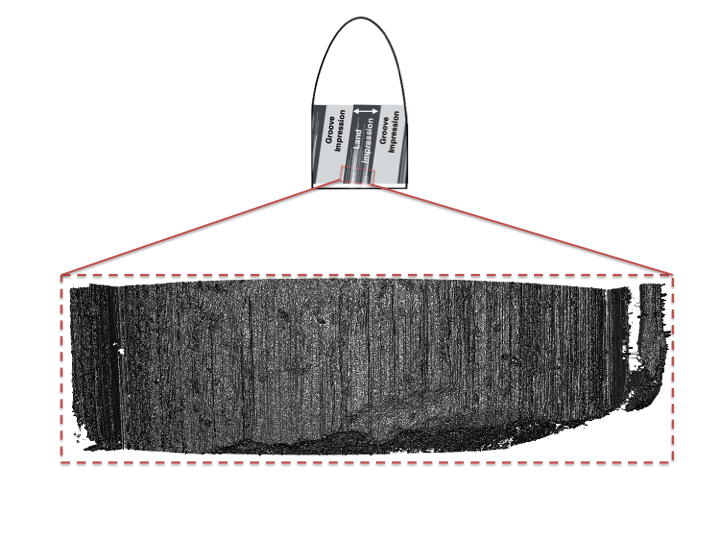
\includegraphics[width=\textwidth]{../images/3d_plot_top_context_breakoff.png}
\caption{An example of an LEA scan from Hamby set 44. There are six LEAs on each bullet in all three test sets.}
\label{LEA-scan}
\end{figure}

The 3D scans of each test set were captured with a Sensofar Confocal
light microscope at 20x magnification resulting in a resolution of 0.645
microns per pixel. These LEAs were scanned at Iowa State University's
High Resolution Microscopy Facility, and the scans are stored in 3D
format as x3p files, conforming to the ISO5436-2 standard
\citep{ISO5436}. A visualization of the data gathered for a single LEA
is seen in \autoref{LEA-scan}. Physically, each land is approximately 2
millimeters in width; as such, data structures for a single LEA can
contain more than 3 million individual data points.

A crosscut was extracted from each scan by identifying an optimal
crosscut using \texttt{x3p\_crosscut\_optimize} in the
\texttt{bulletxtrctr} package in \texttt{R}. Then, an averaged crosscut
was calculated by averaging across ten consecutive crosscuts which fall
directly to either side of the optimal crosscut identified. Shoulder
location methods are applied to these averaged crosscut, for a total of
820 crosscuts across the three test sets.

\section{Methodology}

We first need to remove the global structure of the bullet land.

\subsection{Global Structure Removal}

The non-traditional data structure necessitates employing
non-traditional methods to model and remove the global structure. The
data are made up of two competing structures: the LEA data, of which we
would like to model the global structure, and the GEA data, which we
would like to consider as outlying data. Traditional statistical
modeling techniques minimize the least squared vertical distance from
each data point to a fit line; this results in undue influence by GEA
points, which pull any fit lines towards their unusual points.

While bullets are traditionally circular, it is unwise to use a rigidly
quadratic model to fit the global structure. We cannot assume that fired
bullets will retain a neatly circular shape, especially at the level of
detail scans are captured. The significant amount of physical pressure
that acts upon bullets as they are fired through a barrel also can lead
to some warping or slight deformations \emph{(find a citation from JFS
or AFTE about warping/deformation of bullets?)}. Finally, the placement
of the land relative to the plane of reference when a 3D scan is being
captured can vary slightly, meaning that the 2D crosscuts can be
slightly tilted or rotated. This will not translate into a clean
quadratic-shaped(?) crosscut.

To avoid the potential risks arising from using a quadratic linear
model, we instead use a locally weighted regression (LOESS) which fits
linear regression models on small pieces of the data and combines
predictions to result in a non-parametric predicted fit of the data
structure.

However, since LOESS is still rooted in traditional regression
techniques, it is unable to adequately identify and address the
separation between GEA and LEA data structures. To address this, we
implement a robust version of LOESS which iteratively downweights
unusual data points and re-fits a LOESS model to each land. This robust
LOESS is an adapted version of the robust LOESS proposed by
\cite{Cleveland1}.

This model is fit as follows: (add more formulaic language here\ldots{})

\begin{enumerate}

\item Fit a LOESS model (span = 1) to an entire crosscut to predict y using values of x. Assign weights of 1 to each data point for this fitting procedure.  
\item Obtain predicted values of y from the model fit in step 1.  
\item Calculate residual values using the predicted y values.  
\item Calculate bisquare weights for each residual value using the following formula:  
$$\max(1 - (residual/(6*MAR))^2, 0)^2,$$   where MAR is the median absolute residual for the crosscut.  
\item Assign weights to each data point according to its residual value. If the residual value is positive, assign the bisquare downweight. If the residual is zero or negative, leave the weight at 1.  
\item Repeat steps 1-5 with updated weights at each iteration for $k$ iterations, with 20 iterations as the default.  
\item After $k$ iterations of updating the weight vector, fit a LOESS model (span = 1) and obtained predicted and residual values.  

\end{enumerate}

The subsequent prediction methods for shoulder location are based on the
residuals calculated from the fit to the global structure of each land.
One method uses penalized two-class classification techniques to
classify each data point into ``LEA'' or ``GEA'', while the second uses
Bayesian changepoint analysis to predict the data points at which the
shoulders begin on either side.

\subsection{Two-Class Classification}

Shoulder location can be predicted by classifying data points as one of
two classes: ``LEA'' or ``GEA''. A shoulder location prediction can then
be found by gathering the range of values classified as ``LEA'' points.

Classification into ``LEA'' or ``GEA'' was accomplished by a process of
feature engineering (calculating new variables based on the residuals)
and LASSO regression, a statistical learning method which penalizes the
model for having many large parameters, and thus works to reduce the
overall number of model parameters needed.

The following features are used in the LASSO model:

\begin{itemize}

\item[] \textbf{rlo\_resid\_std}: Robust LOESS residual value, standardized by dividing by standard deviation of residual values from middle 50\% of \textbf{x} values.  

\item[] \textbf{(rlo\_resid\_std$\mathbf{)^2}$}: Squared term of \textbf{rlo\_resid\_std}.  

\item[] \textbf{side}: Whether data point is to left or right of median \textbf{x} value.  

\item[] \textbf{depth\_std}: Distance of data point from median \textbf{x} value, standardized by dividing by maximum \textbf{x} value (a proxy for the range of \textbf{x}).  

\item[] \textbf{side:depth\_std}: Interaction between \textbf{side} and \textbf{depth\_std} variables.  

\item[] \textbf{xint1\_std}: Predicted x intercept of robust LOESS on left side of land, standardized by dividing by maximum \textbf{x} value (a proxy for the range of \textbf{x}).  

\item[] \textbf{xint2\_std}: Predicted x intercept of robust LOESS on right side of land, standardized by dividing by maximum \textbf{x} value (a proxy for the range of \textbf{x}).  

\item[] \textbf{range\_50\_std}: Range of residual values within a 50-point window around data point, standardized by dividing by standard deviation of residual values from middle 50\% of \textbf{x} values.  

\item[] \textbf{numNA\_50}: Number of missing values within a 50-point window around data point.  

\item[] \textbf{ind\_2mad}: Indicator of whether \textbf{rlo\_resid} is greater than \textbf{2*MAD(rlo\_resid)}.  

\item[] \textbf{numpos\_50}: Number of positive residual values within a 50-point window around data point.  

\item[] \textbf{ind\_edges}: Indicator of whether data point is to the left of \textbf{xint1} or to the right of \textbf{xint2}. Values between \textbf{xint1} and \textbf{xint2} receive a value of 0, while values on the outside of the two values receive a value of 1.  

\end{itemize}

Using these features, two separate models were fit: ``LASSO Simple'',
which uses each of the features listed above, and ``LASSO
Interactions'', which uses each of the features along with pairwise
interactions for each of them.

The resulting parameter values for the model fits were used to calculate
predicted values between 0 and 1; the closer to 1, the higher
probability of membership in the ``GEA'' class.

Traditional two-class classification techniques call for finding an
``equal error rate" cutoff to classify the predicted values for each
data point into each of the two classes; i.e., values above a certain
cutoff are classified as part of the ``GEA'' class, and values below the
cutoff are classified as part of the ``LEA'' class. However, since scans
are primarily of the land engraved area, there are many more responses
in the ``LEA'' category than in the ``GEA'' category. This unbalanced
response means that any criterion used to determine a reasonable cutoff
value for classification needs to be adjusted to account for differences
in the size of the response classes.

Thus, instead of looking for the cutoff that gives raw equal error rate
(where sensitivity and specificity are equal), we looked for an equal
error rate based on the overall number of data points. This allows for
an equal \emph{number} of errors in each category, rather than equal
\emph{percentage} of errors. This tactic more fairly penalizes points
that should be classified ``GEA'' but are predicted to be ``LEA''. Due
to the larger class size of ``LEA'', an equal error rate would allow for
more false negatives (i.e., more ``GEA'' data points being classified as
``LEA'') - exactly what we are trying to avoid.

This process results in two methods for groove identification in the
\texttt{bulletxtrctr} package: ``lassobasic'' and ``lassofull''.

\subsection{Bayesian Changepoint Analysis}

The idea behind the changepoint approach is that within either the left
GEA, right GEA, or the LEA, the global structure is consistent and can
either be described by a line with zero slope, a line with positive
slope for the right GEA, or a line with negative slope for the left GEA.
Finding the points where the GEAs and LEA meet is treated as a problem
of model selection. That is, the best fitting statistical model, in
terms of the magnitude of the likelihood, should be the one which
assumes that the points at which the global structure changes align with
where the GEAs and LEA meet. This approach was proposed in the more
general context of Bayesian changepoint detection in
\citet{stephens1994}. Thus, the points of global structural change are
what we will call changepoints. Thus, our model will be defined in a
piecewise fashion. In practice there are also complex additional
patterns which may exist for a number of reasons, but this large scale
structural assumption remains generally reasonable. The complex smaller
scale patterns can be thought of as the dependence in the data after
accounting for the global structure. Because of the nature of the model
which we consider, it becomes necessary for computational reasons to
perform a couple of additional data preprocessing steps. Specifically,
we will scale the residuals from the robust LOESS procedure, and we will
impute missing values. In the next section, we describe the model that
we will use to identify changepoints, after which we will describe the
estimation procedure which we use. Details of the additional data
preprocessing steps can be found in the appendix.

\subsubsection{Bayesian Model Formulation}

Before introducing the model, we introduce some notation. First, let
\(\{Y(x_i): i = 1,2, ..., n\}\) denote the set of random variables
representing the residuals from the robust LOESS procedure at the values
\(x_i\). For simplicity, also assume that \(x_1 < x_2 < ... < x_n\).
Also, let \(c_l\) be the value of the left changepoint and \(c_r\) be
the value of the right changepoint. Here, the left changepoint is where
the left GEA meets the LEA, and the right changepoint is where the right
GEA meets the LEA. Also, denote the median centered \(x\) values as
\(x'_i = x_i - \tilde{x}\) where \(\tilde{x}\) is the median \(x\)
value. As mentioned in the previous paragraph, the complex small scale
patterns, such as the striae, will be modeled through a covariance
structure on the data that will be allowed to differ between each GEA
and between the GEAs and LEA. We will construct the covariance matrices
from the exponential covariance function
\(K(x, x';\sigma, \ell) = \sigma^2 e^{-\frac{|x - x'|}{\ell}} = cov(Y(x), Y(x'))\).
The differences in covariance matrices for the GEAs and LEA will be
reflected in the parameters \(\sigma\) and \(\ell\). The data model that
we consider is then,

\begin{align}
(Y(x_1), Y(x_2), ..., Y(x_{k_1}))^{\top} &\sim N(\beta_{01}\mathbbm{1} + \beta_{11} x_{1:k_1}, \Sigma_1(\sigma_1, \ell_1)) \\
(Y(x_{k_1 + 1}), Y(x_{k_1 + 2}), ..., Y(x_{k_2}))^{\top} &\sim N(0, \Sigma_2(\sigma_2, \ell_2)) \\ 
(Y(x_{k_2 + 1}), Y(x_{k_2 + 2}), ..., Y(x_n))^{\top} &\sim N(\beta_{02}\mathbbm{1} + \beta_{12} x_{k_2 + 1:n}, \Sigma_3(\sigma_3, \ell_3)),
\end{align}

\noindent where \(x_{k_1} < c_l \leq x_{k_1 + 1}\) and
\(x_{k_2} < c_r \leq x_{k_2 + 1}\) Here, \(x_{1:k}\) denotes the column
vector \((x_1, x_2, ..., x_k)^\top\), and \(\mathbbm{1}\) denotes the
vector of ones. Indpendence is assumed between each of these three
distributions for simplicity. The parameters that need to be estimated
include the four mean parameters in the GEAs, the six covariance
parameters (two for each of the three areas), and the two changepoint
parameters, \(c_l\) and \(c_r\).

The above model encapsulates the essence of the approach. However, there
are a few difficulties. The first difficulty is that there are not
always two GEAs in a particular land. There may be one GEA, or the land
may only consist of the LEA. Thus, the above model is actually
conditional on there being two GEAs in the data. We also define models
for when there is one GEA on the left, one GEA on the right, or no GEAs.
The models are defined in an essentially identical way. Conditional on
there being only one GEA, the left GEA model is defined as,

\begin{align}
(Y(x_1), Y(x_2), ..., Y(x_{k}))^{\top} &\sim N(\beta_{0}\mathbbm{1} + \beta_{1} x_{1:k}, \Sigma_1(\sigma_1, \ell_1)) \\
(Y(x_{k + 1}), Y(x_{k + 2}), ..., Y(x_{n}))^{\top} &\sim N(0, \Sigma_2(\sigma_2, \ell_2)),
\end{align}

\noindent and the right GEA model is defined as,

\begin{align}
(Y(x_{1}), Y(x_{2}), ..., Y(x_{k}))^{\top} &\sim N(0, \Sigma_1(\sigma_1, \ell_1)) \\ 
(Y(x_{k + 1}), Y(x_{k + 2}), ..., Y(x_n))^{\top} &\sim N(\beta_{0}\mathbbm{1} + \beta_{1} x_{k + 1:n} \Sigma_2(\sigma_2, \ell_2)).
\end{align}

\noindent Finally, conditional on there being no GEAs in the data, the
model is simply

\begin{align}
(Y(x_{1}), Y(x_{2}), ..., Y(x_{n}))^{\top} &\sim N(0, \Sigma(\sigma, \ell)).
\end{align}

We see that estimating the changepoint locations also involves selecting
the most appropriate model. In order to avoid confusion, we have
slightly abused notation and, for example,
\(\Sigma_1(\sigma_1, \ell_1)\) as it is estimated in the two changepoint
model is \emph{not} the same as \(\Sigma_1(\sigma_1, \ell_1)\) from
either of the one changepoint models, and \(\Sigma_1(\sigma_1, \ell_1)\)
is also \emph{not} the same between the two one changepoint models. As
another example, \(\beta_0\) is \emph{not} the same between each of the
one changepoint models. So, to be clear, duplication of notation in
\emph{different} models is not meant to imply that those parameters are
shared between models.

Ultimately, these above four models are each individually fitted, and
each model above is given a prior. From there, we do model selection in
the formal Bayesian way, selecting number and location of changepoints
by maximizing the estimated posterior distribution.

In order to complete a Bayesian model specification, we need priors on
each of the parameters in each model as well as each model itself. We
will assume independence between each parameter a priori. For each
length scale \(\ell\), we will assume \(\ell \sim \text{Gamma}(3,5)\).
For each standard deviation, we will assume
\(\sigma \sim \text{Half-Normal}^{+}(0,1)\), where
\(\text{Half-Normal}^{+}(\cdot,\cdot)\) is notation for the normal
distribution restricted to the positive real numbers. For intercept
parameters, \(\beta_{01}, \beta_{02}, \beta_0 \sim N(0, 10)\). For the
slope parameters, the preceding trend deviates slightly. For any slope
that corresponds to the \emph{left} GEA, \(\beta_1\) or \(\beta_{01}\),
we will assume that the slope can not be positive. That is,
\(\beta_1, \beta_{01} \sim \text{Half-Normal}^{-}(0,10)\), where
\(\text{Half-Normal}^{-}(\cdot, \cdot)\) is notation for the normal
distribution restricted to the negative real numbers. Contrastingly, for
any slope that corresponds to the \emph{right} GEA, \(\beta_1\) or
\(\beta_{02}\), we will assume that the slope can not be negative. That
is, \(\beta_1, \beta_{01} \sim \text{Half-Normal}^{+}(0,10)\). For the
changepoint locations, we assume a uniform prior
\(\pi(c_l, c_r) \propto I(a < c_l < c_r - \gamma < b - \gamma)\). Here,
\(a\) and \(b\) are some values close to the edges of the data. How
close those values are to the edges is a parameter that is set manually.
Further, we include another hyperparameter, \(\gamma\), which can be set
so that the changepoints are not allowed to be too close to each other.
This is also a parameter that is set manually. Lastly, we assume a
uniform prior over all four models.

\subsubsection{Bayesian Model Estimation}

As was noted in \citet{stephens1994}, for any model including a
changepoint, the likelihood is not a smooth function of the changepoint
location. This is because, holding all other parameters fixed, shifting
the changepoint value will result in zero change to the likelihood until
it crosses the nearest point to the right or left, at which point the
likelihood makes a jump. This makes maximum likelihood estimation in the
standard way infeasible, but Bayesian estimation can be done in a fairly
straightforward way via Markov chain Monte Carlo (MCMC). The basic idea
is that, for each model, we can construct a two step Gibbs sampler. In
step 1 we sample from the posterior distribution of the mean and
covariance parameters given the changepoint locations, and in step 2 we
sample from the changepoint locations given the mean and covariance
parameters. Because of the non-conjugacy in our model, we perform both
sampling steps using a random walk Metropolis-Hastings (RWMH) step with
Gaussian proposals. For details on Gibbs sampling and the
Metropolis-Hastings algorithm see \citet{gelman2013}. It is also worth
mentioning that the zero changepoint model does not require Gibbs
sampling at all, and we perform estimation there using a RWMH algorithm.

We now provide the two basic steps of the Gibbs sampler for the two
changepoint case. The algorithms to sample from the other three models
are omitted, and are nearly identical except for the a smaller number of
parameters need to be sampled. Denote collection of mean and covariance
parameters for the left GEA as \(\theta_1\), the LEA as \(\theta_2\),
and the right GEA as \(\theta_3\). Then, at iteration \(t\) after warmup

\begin{enumerate}
\def\labelenumi{\arabic{enumi}.}
\tightlist
\item
  given changepoint locations \((c_l^{(t - 1)}, c_r^{(t - 1)})\), sample
  \((\theta_1^{(t)}, \theta_2^{(t)}, \theta_3^{(t)})\) using independent
  RWMH steps for each \(\theta_i\)
\item
  given \((\theta_1^{(t)}, \theta_2^{(t)}, \theta_3^{(t)})\), sample
  \((c_l^{(t)}, c_r^{(t)})\) using a single RWMH step.
\end{enumerate}

After running the MCMC for each model, parameter estimates and the most
likely model are jointly chosen according to the largest joint posterior
value. That is, we arrive at estimates
\((\hat{\theta}, \hat{M}) = \underset{(\theta, M)}{\operatorname{argmax}}{\log(p(\theta, M | Y))}\),
where \(M\) is the random variable associated with the choice of model,
\(\theta\) is the associated parameter vector for the appropriate model,
and \(Y\) is all of the available data. Additional MCMC details can be
found in the appendix.

The idea behind the changepoint approach is that within either the left
GEA, right GEA, or the LEA, the global structure is consistent and can
either be described by a line with zero slope, a line with positive
slope for the right GEA, or a line with negative slope for the left GEA.
Finding the points where the GEAs and LEA meet is treated as a problem
of model selection. That is, the best fitting statistical model, in
terms of the magnitude of the likelihood, should be the one which
assumes that the points at which the global structure changes align with
where the GEAs and LEA meet. This approach was proposed in the more
general context of Bayesian changepoint detection in
\citet{stephens1994}. Thus, the points of global structural change are
what we will call changepoints. Thus, our model will be defined in a
piecewise fashion. In practice there are also complex additional
patterns which may exist for a number of reasons, but this large scale
structural assumption remains generally reasonable. The complex smaller
scale patterns can be thought of as the dependence in the data after
accounting for the global structure. Because of the nature of the model
which we consider, it becomes necessary for computational reasons to
perform a couple of additional data preprocessing steps. Specifically,
we will scale the residuals from the robust LOESS procedure, and we will
impute missing values. In the next section, we describe the model that
we will use to identify changepoints, after which we will describe the
estimation procedure which we use. Details of the additional data
preprocessing steps can be found in the appendix.

\subsubsection{Bayesian Model Formulation}

Before introducing the model, we introduce some notation. First, let
\(\{Y(x_i): i = 1,2, ..., n\}\) denote the set of random variables
representing the residuals from the robust LOESS procedure at the values
\(x_i\). For simplicity, also assume that \(x_1 < x_2 < ... < x_n\).
Also, let \(c_l\) be the value of the left changepoint and \(c_r\) be
the value of the right changepoint. Here, the left changepoint is where
the left GEA meets the LEA, and the right changepoint is where the right
GEA meets the LEA. Also, denote the median centered \(x\) values as
\(x'_i = x_i - \tilde{x}\) where \(\tilde{x}\) is the median \(x\)
value. As mentioned in the previous paragraph, the complex small scale
patterns, such as the striae, will be modeled through a covariance
structure on the data that will be allowed to differ between each GEA
and between the GEAs and LEA. We will construct the covariance matrices
from the exponential covariance function
\(K(x, x';\sigma, \ell) = \sigma^2 e^{-\frac{|x - x'|}{\ell}} = cov(Y(x), Y(x'))\).
The differences in covariance matrices for the GEAs and LEA will be
reflected in the parameters \(\sigma\) and \(\ell\). The data model that
we consider is then,

\begin{align}
(Y(x_1), Y(x_2), ..., Y(x_{k_1}))^{\top} &\sim N(\beta_{01}\mathbbm{1} + \beta_{11} x_{1:k_1}, \Sigma_1(\sigma_1, \ell_1)) \\
(Y(x_{k_1 + 1}), Y(x_{k_1 + 2}), ..., Y(x_{k_2}))^{\top} &\sim N(0, \Sigma_2(\sigma_2, \ell_2)) \\ 
(Y(x_{k_2 + 1}), Y(x_{k_2 + 2}), ..., Y(x_n))^{\top} &\sim N(\beta_{02}\mathbbm{1} + \beta_{12} x_{k_2 + 1:n}, \Sigma_3(\sigma_3, \ell_3)),
\end{align}

\noindent where \(x_{k_1} < c_l \leq x_{k_1 + 1}\) and
\(x_{k_2} < c_r \leq x_{k_2 + 1}\) Here, \(x_{1:k}\) denotes the column
vector \((x_1, x_2, ..., x_k)^\top\), and \(\mathbbm{1}\) denotes the
vector of ones. Indpendence is assumed between each of these three
distributions for simplicity. The parameters that need to be estimated
include the four mean parameters in the GEAs, the six covariance
parameters (two for each of the three areas), and the two changepoint
parameters, \(c_l\) and \(c_r\).

The above model encapsulates the essence of the approach. However, there
are a few difficulties. The first difficulty is that there are not
always two GEAs in a particular land. There may be one GEA, or the land
may only consist of the LEA. Thus, the above model is actually
conditional on there being two GEAs in the data. We also define models
for when there is one GEA on the left, one GEA on the right, or no GEAs.
The models are defined in an essentially identical way. Conditional on
there being only one GEA, the left GEA model is defined as,

\begin{align}
(Y(x_1), Y(x_2), ..., Y(x_{k}))^{\top} &\sim N(\beta_{0}\mathbbm{1} + \beta_{1} x_{1:k}, \Sigma_1(\sigma_1, \ell_1)) \\
(Y(x_{k + 1}), Y(x_{k + 2}), ..., Y(x_{n}))^{\top} &\sim N(0, \Sigma_2(\sigma_2, \ell_2)),
\end{align}

\noindent and the right GEA model is defined as,

\begin{align}
(Y(x_{1}), Y(x_{2}), ..., Y(x_{k}))^{\top} &\sim N(0, \Sigma_1(\sigma_1, \ell_1)) \\ 
(Y(x_{k + 1}), Y(x_{k + 2}), ..., Y(x_n))^{\top} &\sim N(\beta_{0}\mathbbm{1} + \beta_{1} x_{k + 1:n} \Sigma_2(\sigma_2, \ell_2)).
\end{align}

\noindent Finally, conditional on there being no GEAs in the data, the
model is simply

\begin{align}
(Y(x_{1}), Y(x_{2}), ..., Y(x_{n}))^{\top} &\sim N(0, \Sigma(\sigma, \ell)).
\end{align}

We see that estimating the changepoint locations also involves selecting
the most appropriate model. In order to avoid confusion, we have
slightly abused notation and, for example,
\(\Sigma_1(\sigma_1, \ell_1)\) as it is estimated in the two changepoint
model is \emph{not} the same as \(\Sigma_1(\sigma_1, \ell_1)\) from
either of the one changepoint models, and \(\Sigma_1(\sigma_1, \ell_1)\)
is also \emph{not} the same between the two one changepoint models. As
another example, \(\beta_0\) is \emph{not} the same between each of the
one changepoint models. So, to be clear, duplication of notation in
\emph{different} models is not meant to imply that those parameters are
shared between models.

Ultimately, these above four models are each individually fitted, and
each model above is given a prior. From there, we do model selection in
the formal Bayesian way, selecting number and location of changepoints
by maximizing the estimated posterior distribution.

In order to complete a Bayesian model specification, we need priors on
each of the parameters in each model as well as each model itself. We
will assume independence between each parameter a priori. For each
length scale \(\ell\), we will assume \(\ell \sim \text{Gamma}(3,5)\).
For each standard deviation, we will assume
\(\sigma \sim \text{Half-Normal}^{+}(0,1)\), where
\(\text{Half-Normal}^{+}(\cdot,\cdot)\) is notation for the normal
distribution restricted to the positive real numbers. For intercept
parameters, \(\beta_{01}, \beta_{02}, \beta_0 \sim N(0, 10)\). For the
slope parameters, the preceding trend deviates slightly. For any slope
that corresponds to the \emph{left} GEA, \(\beta_1\) or \(\beta_{01}\),
we will assume that the slope can not be positive. That is,
\(\beta_1, \beta_{01} \sim \text{Half-Normal}^{-}(0,10)\), where
\(\text{Half-Normal}^{-}(\cdot, \cdot)\) is notation for the normal
distribution restricted to the negative real numbers. Contrastingly, for
any slope that corresponds to the \emph{right} GEA, \(\beta_1\) or
\(\beta_{02}\), we will assume that the slope can not be negative. That
is, \(\beta_1, \beta_{01} \sim \text{Half-Normal}^{+}(0,10)\). For the
changepoint locations, we assume a uniform prior
\(\pi(c_l, c_r) \propto I(a < c_l < c_r - \gamma < b - \gamma)\). Here,
\(a\) and \(b\) are some values close to the edges of the data. How
close those values are to the edges is a parameter that is set manually.
Further, we include another hyperparameter, \(\gamma\), which can be set
so that the changepoints are not allowed to be too close to each other.
This is also a parameter that is set manually. Lastly, we assume a
uniform prior over all four models.

\subsubsection{Bayesian Model Estimation}

As was noted in \citet{stephens1994}, for any model including a
changepoint, the likelihood is not a smooth function of the changepoint
location. This is because, holding all other parameters fixed, shifting
the changepoint value will result in zero change to the likelihood until
it crosses the nearest point to the right or left, at which point the
likelihood makes a jump. This makes maximum likelihood estimation in the
standard way infeasible, but Bayesian estimation can be done in a fairly
straightforward way via Markov chain Monte Carlo (MCMC). The basic idea
is that, for each model, we can construct a two step Gibbs sampler. In
step 1 we sample from the posterior distribution of the mean and
covariance parameters given the changepoint locations, and in step 2 we
sample from the changepoint locations given the mean and covariance
parameters. Because of the non-conjugacy in our model, we perform both
sampling steps using a random walk Metropolis-Hastings (RWMH) step with
Gaussian proposals. For details on Gibbs sampling and the
Metropolis-Hastings algorithm see \citet{gelman2013}. It is also worth
mentioning that the zero changepoint model does not require Gibbs
sampling at all, and we perform estimation there using a RWMH algorithm.

We now provide the two basic steps of the Gibbs sampler for the two
changepoint case. The algorithms to sample from the other three models
are omitted, and are nearly identical except for the a smaller number of
parameters need to be sampled. Denote collection of mean and covariance
parameters for the left GEA as \(\theta_1\), the LEA as \(\theta_2\),
and the right GEA as \(\theta_3\). Then, at iteration \(t\) after warmup

\begin{enumerate}
\def\labelenumi{\arabic{enumi}.}
\tightlist
\item
  given changepoint locations \((c_l^{(t - 1)}, c_r^{(t - 1)})\), sample
  \((\theta_1^{(t)}, \theta_2^{(t)}, \theta_3^{(t)})\) using independent
  RWMH steps for each \(\theta_i\)\\
\item
  given \((\theta_1^{(t)}, \theta_2^{(t)}, \theta_3^{(t)})\), sample
  \((c_l^{(t)}, c_r^{(t)})\) using a single RWMH step.
\end{enumerate}

After running the MCMC for each model, parameter estimates and the most
likely model are jointly chosen according to the largest joint posterior
value. That is, we arrive at estimates
\((\hat{\theta}, \hat{M}) = \underset{(\theta, M)}{\operatorname{argmax}}{\log(p(\theta, M | Y))}\),
where \(M\) is the random variable associated with the choice of model,
\(\theta\) is the associated parameter vector for the appropriate model,
and \(Y\) is all of the available data. Additional MCMC details can be
found in the appendix.

\section{Results}

\subsection{Hamby set 44}

\begin{table}[]
\centering
\caption{Downstream results for Hamby set 44}
\begin{tabular}{lllllll}
& & \multicolumn{5}{c}{\textbf{Controlled FPR = .01}}\\
\textbf{Method} & \textbf{AUC} & Cutoff & FN &TP & TN & Accuracy \\ \hline
Rollapply & 0.8 &  0.92 & 332 & 420&42126 & 0.98 \\ \hline
LASSO basic & 0.94 &  0.75 &126 & 626&42098 & 0.99\\ \hline
LASSO full & 0.94 &  0.75 &126 &626 &42106 & 0.99 \\ \hline
Bayesian Changepoint & 0.93 &  0.74 &152 & 600&42098 & 0.99\\ \hline
Manual ID & 0.94 &  0.74 & 124& 628&42088 & 0.99\\ \hline 
\end{tabular}
\end{table}

\subsection{Phoenix PD}

\begin{table}[]
\centering
\caption{Downstream results for Phoenix PD set}
\begin{tabular}{lllllll}
& & \multicolumn{5}{c}{\textbf{Controlled FPR = .01}}\\
\textbf{Method} & \textbf{AUC} & Cutoff & FN &TP & TN & Accuracy \\ \hline
Rollapply & 0.818 &  0.9 & 364 & 378&38082 & 0.981 \\ \hline
LASSO basic & 0.877 &  0.947 &256 & 486&38088 & 0.9839\\ \hline
LASSO full & 0.893 &  0.953 &238 &504 &38082 & 0.9842 \\ \hline
Bayesian Changepoint & 0.903 &  0.937 &256 & 486&38080 & 0.9837\\ \hline
Manual ID & 0.953 &  0.853 & 96& 646&38084 & 0.9879\\ \hline 
\end{tabular}
\end{table}

\subsection{Houston-test set}

\begin{table}[]
\centering
\caption{Downstream results for Houston-test set}
\begin{tabular}{lllllll}
& & \multicolumn{5}{c}{\textbf{Controlled FPR = .01}}\\
\textbf{Method} & \textbf{AUC} & Cutoff & FN &TP & TN & Accuracy \\ \hline
Rollapply & 0.761 &  0.91 & 1652 & 1016&167118 & 0.981 \\ \hline
LASSO basic & 0.852 &  0.88 &1274 & 1394&167136 & 0.9833\\ \hline
LASSO full & 0.858 &  0.823 &1144 &1524 &167062 & 0.9836 \\ \hline
Bayesian Changepoint & 0.795 &  0.863 &1552 & 1116&167096 & 0.9814\\ \hline
Manual ID & 0.931 &  0.823 & 614& 2054&167098 & 0.9869\\ \hline 
\end{tabular}
\end{table}

\section{Conclusions}

\section{References}

\section{Appendix}

\subsection{MCMC Details}

As a practical note, it turns out that the posterior distribution is
almost always multimodal, and it can happen that the sampler gets stuck
in a suboptimal mode for a large number of iterations. It is also the
case that the suboptimal modes need not even be close to the groove
locations. It has, however, been our experience that the optimal mode
corresponds well to the actual groove locations, which are often
somewhat close to the edges of the data. With this in mind, starting
values and the RWMH proposal variances play a very important role in the
success of the sampling algorithm. Fortunately, it seems to be the case
that by setting the initial changepoint values close to the edges of the
data and making the proposal variance small (around 100 seems to work
well) allows the sampler to wander inwards, and even with a modest
number of iterations (say 5000), typically pass through the largest mode
corresponding to the groove locations. This is not always the case, and
it is possible that increasing the number of iterations produces better
results.

In our implementation of this algorithm, the sampling functions were
originally written with the intention of tuning the proposal variances
to potentially accelerate convergence, and thus several warmup
iterations are required for this purpose. This turns out to be a bad
idea in this context for two reasons. The first reason is that the
warmup iterations allow the sampler to wander past the global modes and
get stuck in suboptimal modes far from the groove locations, from which
the sampler may or may not find its way back to the optimal modes in
just a few thousand iterations. Secondly, if the sampler does wander
past the optimal modes, which are usually on the edges of the data, the
tuned proposal variance can be quite large. The large proposal variance
might not be a huge problem if it weren't for the fact that the width of
the modes are almost always quite small. This means that it can take a
very, very long time for the sampler to move from a suboptimal mode to
the global mode. In order to mitigate this problem, we are currently
setting the number of warmup iterations to be relatively small
(somewhere in 100 to 500 seems to work well). In future, our
implementation of the algorithm will not require any warmup iterations.

Initially, the Metropolis proposal variance for each \(\theta_i\) is
diagonal with diagonal elements all equal to \(1/2\). The proposal
variance for \((c_l, c_r)\) is initially set to be diagonal with
elements equal to \(10^2\). Note that because of the currently necessary
warmup iterations, the variances after warmup for each \(\theta_i\)
becomes
\(\frac{2.4^2}{d}\hat{Var}(\theta_i^{(1:w)}) + \text{diag}(0.1)\), where
\(d\) is the dimension of \(\theta_i\) (which is not constant between
GEAs and LEA), and \(\hat{Var}(\theta_i^{(1:w)})\) is the estimated
variance covariance matrix from the \(w\) warmup iterations. Note that
the addition of a diagonal matrix with entries \(0.1\) is to avoid the
case when most or all warmup iterations have the same value. Similarly,
the proposal variance for \((c_l, c_r)\) after warmup becomes
\(\frac{2.4^2}{2}\hat{Var}((c_l,c_r)^{(1:w)}) + \text{diag}(1)\).

\subsection{Data Preprocessing for MCMC}

Before running the MCMC to do the changepoint detection, we first
perform two data preprocessing steps. The first step is to scale the
residuals from the robust loess procedure by the standard deviation
calculated from the entire set of residuals. The reason for this is
simply to make priors for standard deviation and slope parameters easier
to specify. For example, ensuring that the residuals are scaled to have
standard deviation one means that the standard deviation parameters in
our model should also be close to one. This scaling also ensures that
slopes values are not very large.

The second preprocessing step is a bit more involved. In order to enable
the algorithm to run reasonably fast, we need to take advantage of the
sparse precision matrix structure that is induced by the exponential
covariance function. Indeed, this was the reason for choosing this
covariance function in the first place. Unfortunately, it is challenging
to do this unless the observations are evenly spaced in the domain. In
our case, this would be true if there were no missing values. In order
to remedy this problem, we impute the missing data, but only in the case
that there exist nonmissing observations outside of the missing values.
In the case that the missing values exist on the edges of the data, we
simply do not consider those domain values in the model.

We perform the imputation by treating the observations as coming from an
unknown function, and infer the missing values from the known function
values. In order to do this, we model the data with a Gaussian process
and the squared exponential covariance function. That is, we suppose
that

\[
Y(x) \sim \mathcal{GP}(0, K(x,x';\sigma^2, \ell)),
\]

\noindent where now
\(K(x,x';\sigma^2, \ell) = \sigma^2 e^{-(x - x')^2/(2\ell^2)}\) is the
squared exponential covariance function. We emphasize for clarity that
this is a different covariance function than we use in the changepoint
model. The main reason for this is that in imputing values, it seems
desireable to allow dependencies beyond immediately neighboring points
to influence predictions as the function that we are trying to predict
generally has a smooth global structure. For all of our experiments, we
set \(\sigma = 0.8\) and \(\ell = 15\). These values were chosen from
doing maximum likelihood estimation for a representative bullet.

When we impute the missing values, we compute the conditional mean of
the missing values. To be clear, denote the distribution of the observed
and missing data as

\[ 
(Y,Y^*)^\top \sim N\left( \begin{bmatrix} 0 \\ 0 \end{bmatrix}, \begin{bmatrix} \Sigma_{yy} & \Sigma_{yy^*} \\ \Sigma_{y^*y} & \Sigma_{y^*y^*}\end{bmatrix} \right).
\]

\noindent Here, \(Y\) is observed data and \(Y^*\) is the missing data,
and the covariance matrix above is constructed from the squared
exponential covariance function. We then use normal distribution theory
to calculate the imputed values

\[ E(Y^*|Y = y) = \Sigma_{y^*y} \Sigma_{yy}^{-1}y \].

\bibliographystyle{jfs-authoryear}
\bibliography{bibliography}

\end{document}